\section{Zielsetzung}
Das Ziel dieses Versuches ist die Bestimmung der realen Gütenziffer,
des Massendurchsatzes und der mechanischen Kompressorleitung. Darüberhinaus
sollen diese mit ideal Werten verglichen werden.
\section{Theorie}
\label{sec:Theorie}
\subsection{Prinzip der Wärmepumpe}
Die Wärmeenergie eines geschlossenen Systems geht erfahrungsgemäß immer von
einem wärmerem Medium in ein kälteres über. Laut Energiesatz ist aber auch der
umgekehrte Fall möglich, wenn zusätzliche Energie aufgewendet wird.
Dieses Prinzip findet in einer sogenannten Wärmepumpe seine Anwendung.
Das Verhältnis zwischen der tranportierten Wärmemenge und der so aufgewendeten
Arbeit bezeichnet man als Güteziffer der Wärmpumpe. Unter idealen Vorrausetzungen,
also ohne Wärmeverlust und praktisch keiner Temperaturänderung bei einem
reversiblen Prozess, ist diese Güteziffer $\nu_{id}$ definiert durch:
\begin{equation}
  \nu_{id} = \frac{Q_1}{A} = \frac{T_1}{T_1 - T_2}.
  \label{eqn:idgüte}
\end{equation}
Dabei bezeichnet $Q_1$ die abgegebene Wärmemenge, $A$ die aufgewendete Arbeit,
$T_1$ die Temperatur des Mediums aus dem Wärme abgegeben wird und $T_2$ die
Temperatur in des Mediums in das Wärme gepumpt wird.
\subsection{Funktionsweise einer Wärmepumpe}
Die Wärmepumpe benutzt ein Gas als Transportmedium, dieses Gas nimmt
beim Verdampfen Wärme auf und gibt sie beim Verflüssigen wieder ab. Der
schematische Aufbau der Wärmepumpe der im Folgenden beschrieben wird,
ist in der Abbildung \ref{fig:schema} dargestellt.
Ein Kompressor erzeugt so einen Kreislauf. Das Transportmedium wird so durch
Reservoire 1 und 2 und das Drosselventil gepumpt. Die Wärmepumpe ist so
aufgebaut, dass das Transportmedium bei der Temperatur im Reservoire 1 unter dem
Druck $p_a$ flüssig und bei Temperatur 2 unter dem Druck $p_b$ gasförmig ist.
nach druchströmen des Drosselventils der dampft das flüssige Transportmedium und
entzieht somit dem Reservoire 2 die Verdampfungswärme $L$. Danach wird das
Transportgas adiabatisch komprimiert, dabei erwärmt es sich stark und der Druck
ansteigt, bis es im Reservoire 1 kondensiert. Das führt dazu, dass die
Wärme $L$ an das Reservoire 1 abgegeben wird. Um ein einwandfreies Funktionieren
der Wärmepumpe zu gewährleisten, muss vor dem Drosselventil ein "Reiniger" sein
der das Transportmedium von Gasresten trennt sowie eine Steuerungsvorrichtung für
das Drosselventil. Der genaue Aufbau ist in Abbildung \ref{fig:aufbau} dargestellt.
Die Temperaturen der Reservoirs werden mit Temometern gemessen, um genaue
Temperaturangeaben zu haben wird der Inhalt der Reservoire mit Rührmotoren
umgerührt. Die Reservoirs werden mit der gleiche Menge Wasser aufgefüllt.
\begin{figure}
  \centering
  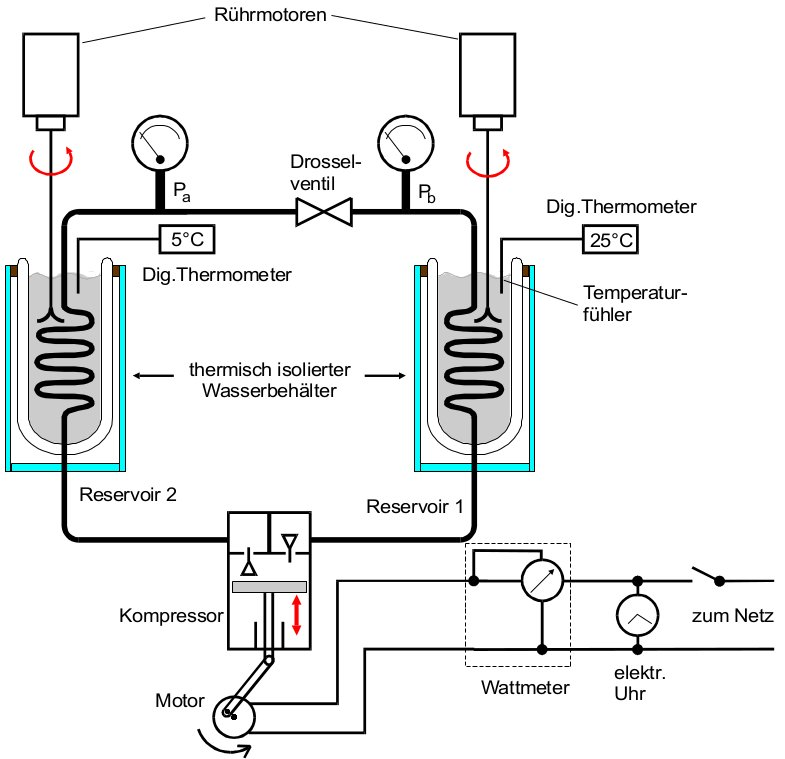
\includegraphics[height=7cm]{logos/AufbauWaermepumpe.jpg}
  \caption{Schematischer Aufbau einer Wärmepumpe \cite{Anleitung}}
  \label{fig:schema}
\end{figure}
\FloatBarrier
\subsection{Kenngrößen einer realen Wärmepumpe}
\subsubsection{Die reale Güteziffer}
Die reale Güteziffer $\nu$ ist definiert als
\begin{equation}
  \nu = \frac{\increment Q_1}{\increment t N}.
  \label{eqn:realGüte}
\end{equation}
Dabei bezeichnet $N$ die über den Zeitraum $\increment t $ gemittelte
Leistungsaufnahme des Kompressors und $\frac{\increment Q_1}{\increment t }$
die gewonnene Wärmemenge pro Zeit. Diese wird berechnet mit
\begin{equation}
  \frac{\increment Q_1}{\increment t} =(m_1 c_w + m_k c_k)
  \frac{\increment T_1}{\increment t}.
  \label{eqn:q1}
\end{equation}
Darin bezeichnet $m_1c_w$ die Wärmekapazität des Wassers im Reservoire 1 und
$m_kc_k$ die Wärmekapazitat der Kupferschlange und des Eimers.
\subsubsection{Bestimmung des Massendurchsatzes}
Der Massendurchsatz lässt sich durch die Gleichung
\begin{equation}
  \frac{\increment Q_2}{\increment t} = L \frac{\increment m}{\increment t}
\end{equation}
berechnen. Die Berechnung von $\frac{\increment Q_2}{\increment t}$ ist dabei
analog zu \eqref{eqn:q1} und die Größe $L$ ist die Verdampfungswärme.
\subsubsection{Bestimmung der Kompressionsleitung \texorpdfstring{$N_{mech}$}{math}}
Die Arbeit $A_m$ um ein Gasvolumen $V_a$ auf $V_b$ zu komprimieren ist geben durch:
\begin{equation}
  A_m = \int_{V_a} ^ {V_b} p \, \symup{d}V.
\end{equation}
Angenommen die Kompression verläuft adiabatisch so folgt
\begin{equation*}
  p_a V_a ^\kappa = p_b V_b ^\kappa = p V^\kappa.
\end{equation*}
Daraus ergibt sich für $A_m$
\begin{equation}
  A_m = \frac{1}{\kappa -1}\left(p_b \sqrt[\kappa]{ \frac{p_a}{p_b}}- p_a
  \right) V_a
\end{equation}
und für $N_{mech}$
\begin{equation}
  N_{mech} = \frac{1}{\kappa -1}\left(p_b \sqrt[\kappa]{ \frac{p_a}{p_b}}- p_a
  \right) \frac{1}{\rho} \frac{\increment m}{\increment t}.
\end{equation}





























%
